\subsubsection{RLPx Transport Protocol}
\label{sec:rlpx-transport-protocol}

The aim of this protocol is to provide a generalized mean to build arbitrary
authenticated and encrypted protocols. Everyone can create a new protocol by 
simply selecting $3$ ASCII characters to uniquely identify the protocol and by
defining a list of packet types and the expected structure of the content, that 
should be encoded with RLP.

\begin{figure}
    \begin{center}
        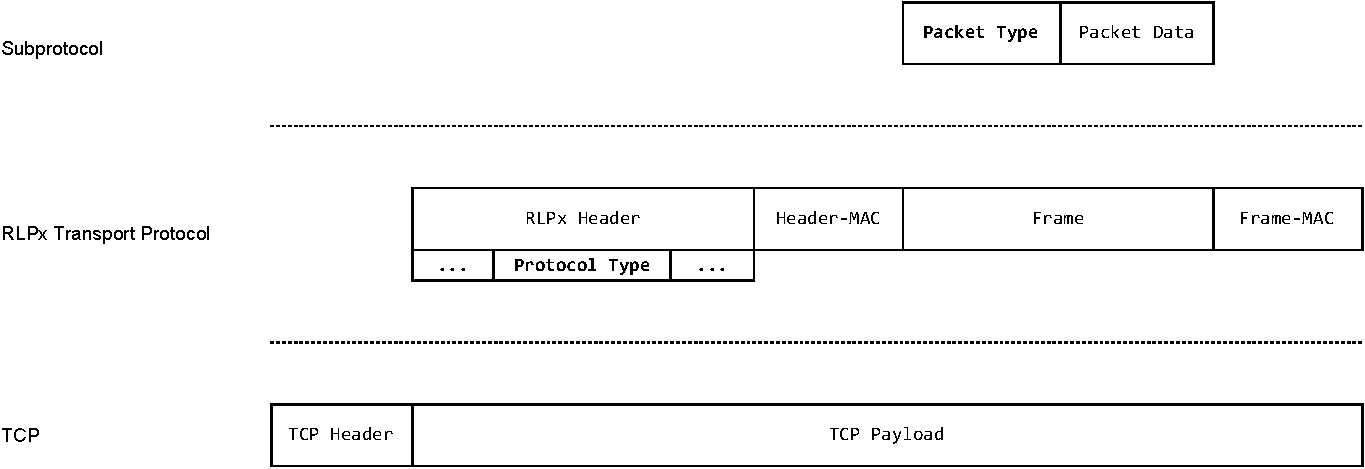
\includegraphics[width=\textwidth]{./res/img/rlpx-transport}
        \caption{Relationship between TCP, RLPx and the subprotocols}
        \label{fig:rlpx-transport}
    \end{center}
\end{figure}

The relationship between TCP, RLPx and the subprotocol and the structure of
these packages is depicted in~\autoref{fig:rlpx-transport}. Although the RLPx
transport protocol can split big packages in frames, we consider here only 
packages with a single frame for the sake of simplicity and refer to interested
readers to the official documentation~\cite{rlpx}.

Concretely, the RLPx transport protocol is built on top of TCP, i.e., it is
sent as payload in a TCP packet. The content of this packet is serialized using 
the RLP marshaling algorithm. The peers who want to communicate with each other 
with RLPx should perform two handshakes:
\begin{enumerate}
    \item Encoding Handshake, it is used to exchange a cryptographic 
    secret\footnote{It is beyond the scope of this report to describe the exact 
    procedure. For further details we refer to the official documentation 
    \cite{rlpx} and to the go Ethereum implementation 
    \url{https://github.com/ethereum/go-ethereum/blob/master/p2p/rlpx.go}.}
    that is used to encrypt and authenticate the subsequent RLPx messages 
    between them.
    \item Protocol Handshake, in which the peers exchanges and agree on the 
    subprotocols and versions, also known as \emph{capabilities}, that both
    support. Essentially, both exchange a \texttt{Hello} message, that contain
    the list of supported subprotocols and their versions. Each one
    independently compute the list of common capabilities, sort it  according 
    to the lexicographic order and identify each pair 
    protocol/version with the index in the list.
\end{enumerate}

